\chapter{Experimentelle Untersuchungen im Windkanal}\label{s:versuche}

\section{Windkanalbeschreibung (KK)}
F"ur die experimentellen Untersuchungen steht der LNB (Leiser Niedergeschwindigkeitskanal Braunschweig) vom Institut f"ur Str"omungsmechanik der technischen  Universit"at Braunschweig zur Verf"ugung.\\
Dieser ist an beiden Enden offen und wird durch die Umgebungsluft im Raum versorgt, was als Eiffel-Bauart bezeichnet wird. (\abb{fig:windkanal}).
Durch eine besondere Art der Polsterung bzw. Schalld"ampfer und einen
ger"auscharmen Elektroantrieb, ist dieser Windkanal so f"ur einen m"oglichst leisen Betrieb konstruiert worden.
\begin{figure}[h]
	\centering
	\begin{subfigure}[c]{0.5\textwidth}		
		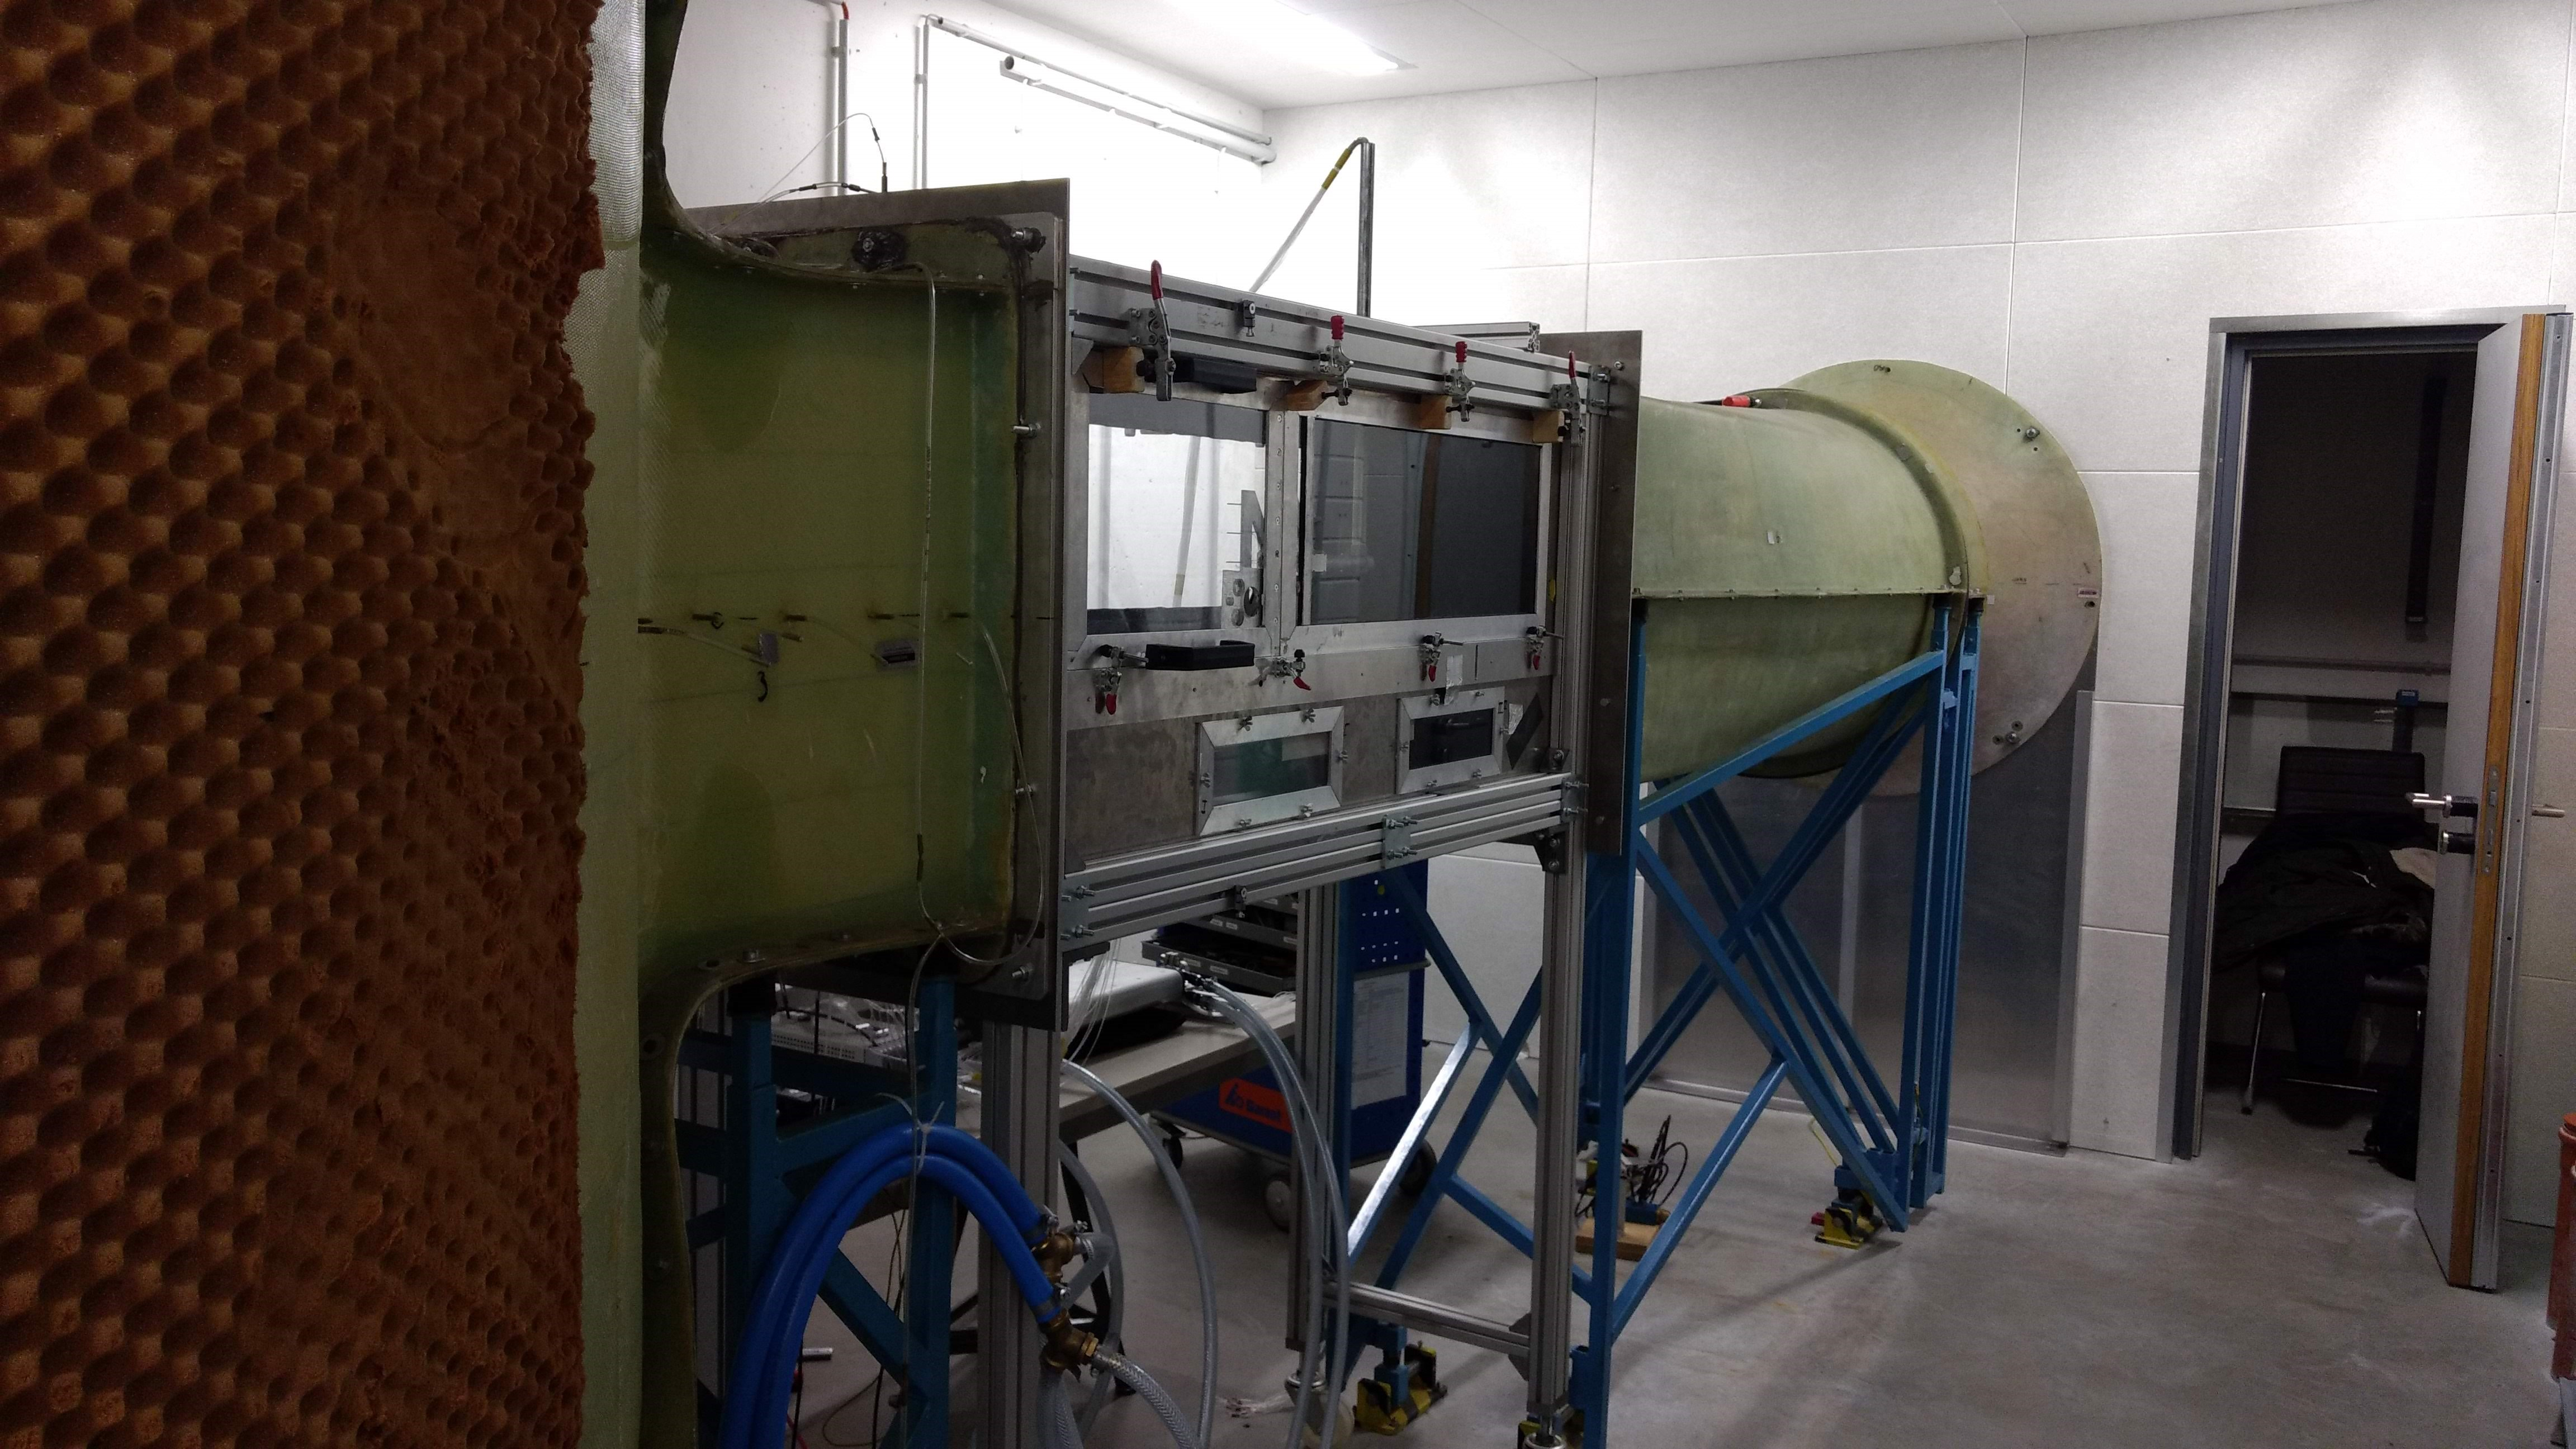
\includegraphics[width=1\textwidth]{windkanal1.jpg}
	\end{subfigure}
	\begin{subfigure}[c]{0.5\textwidth}
		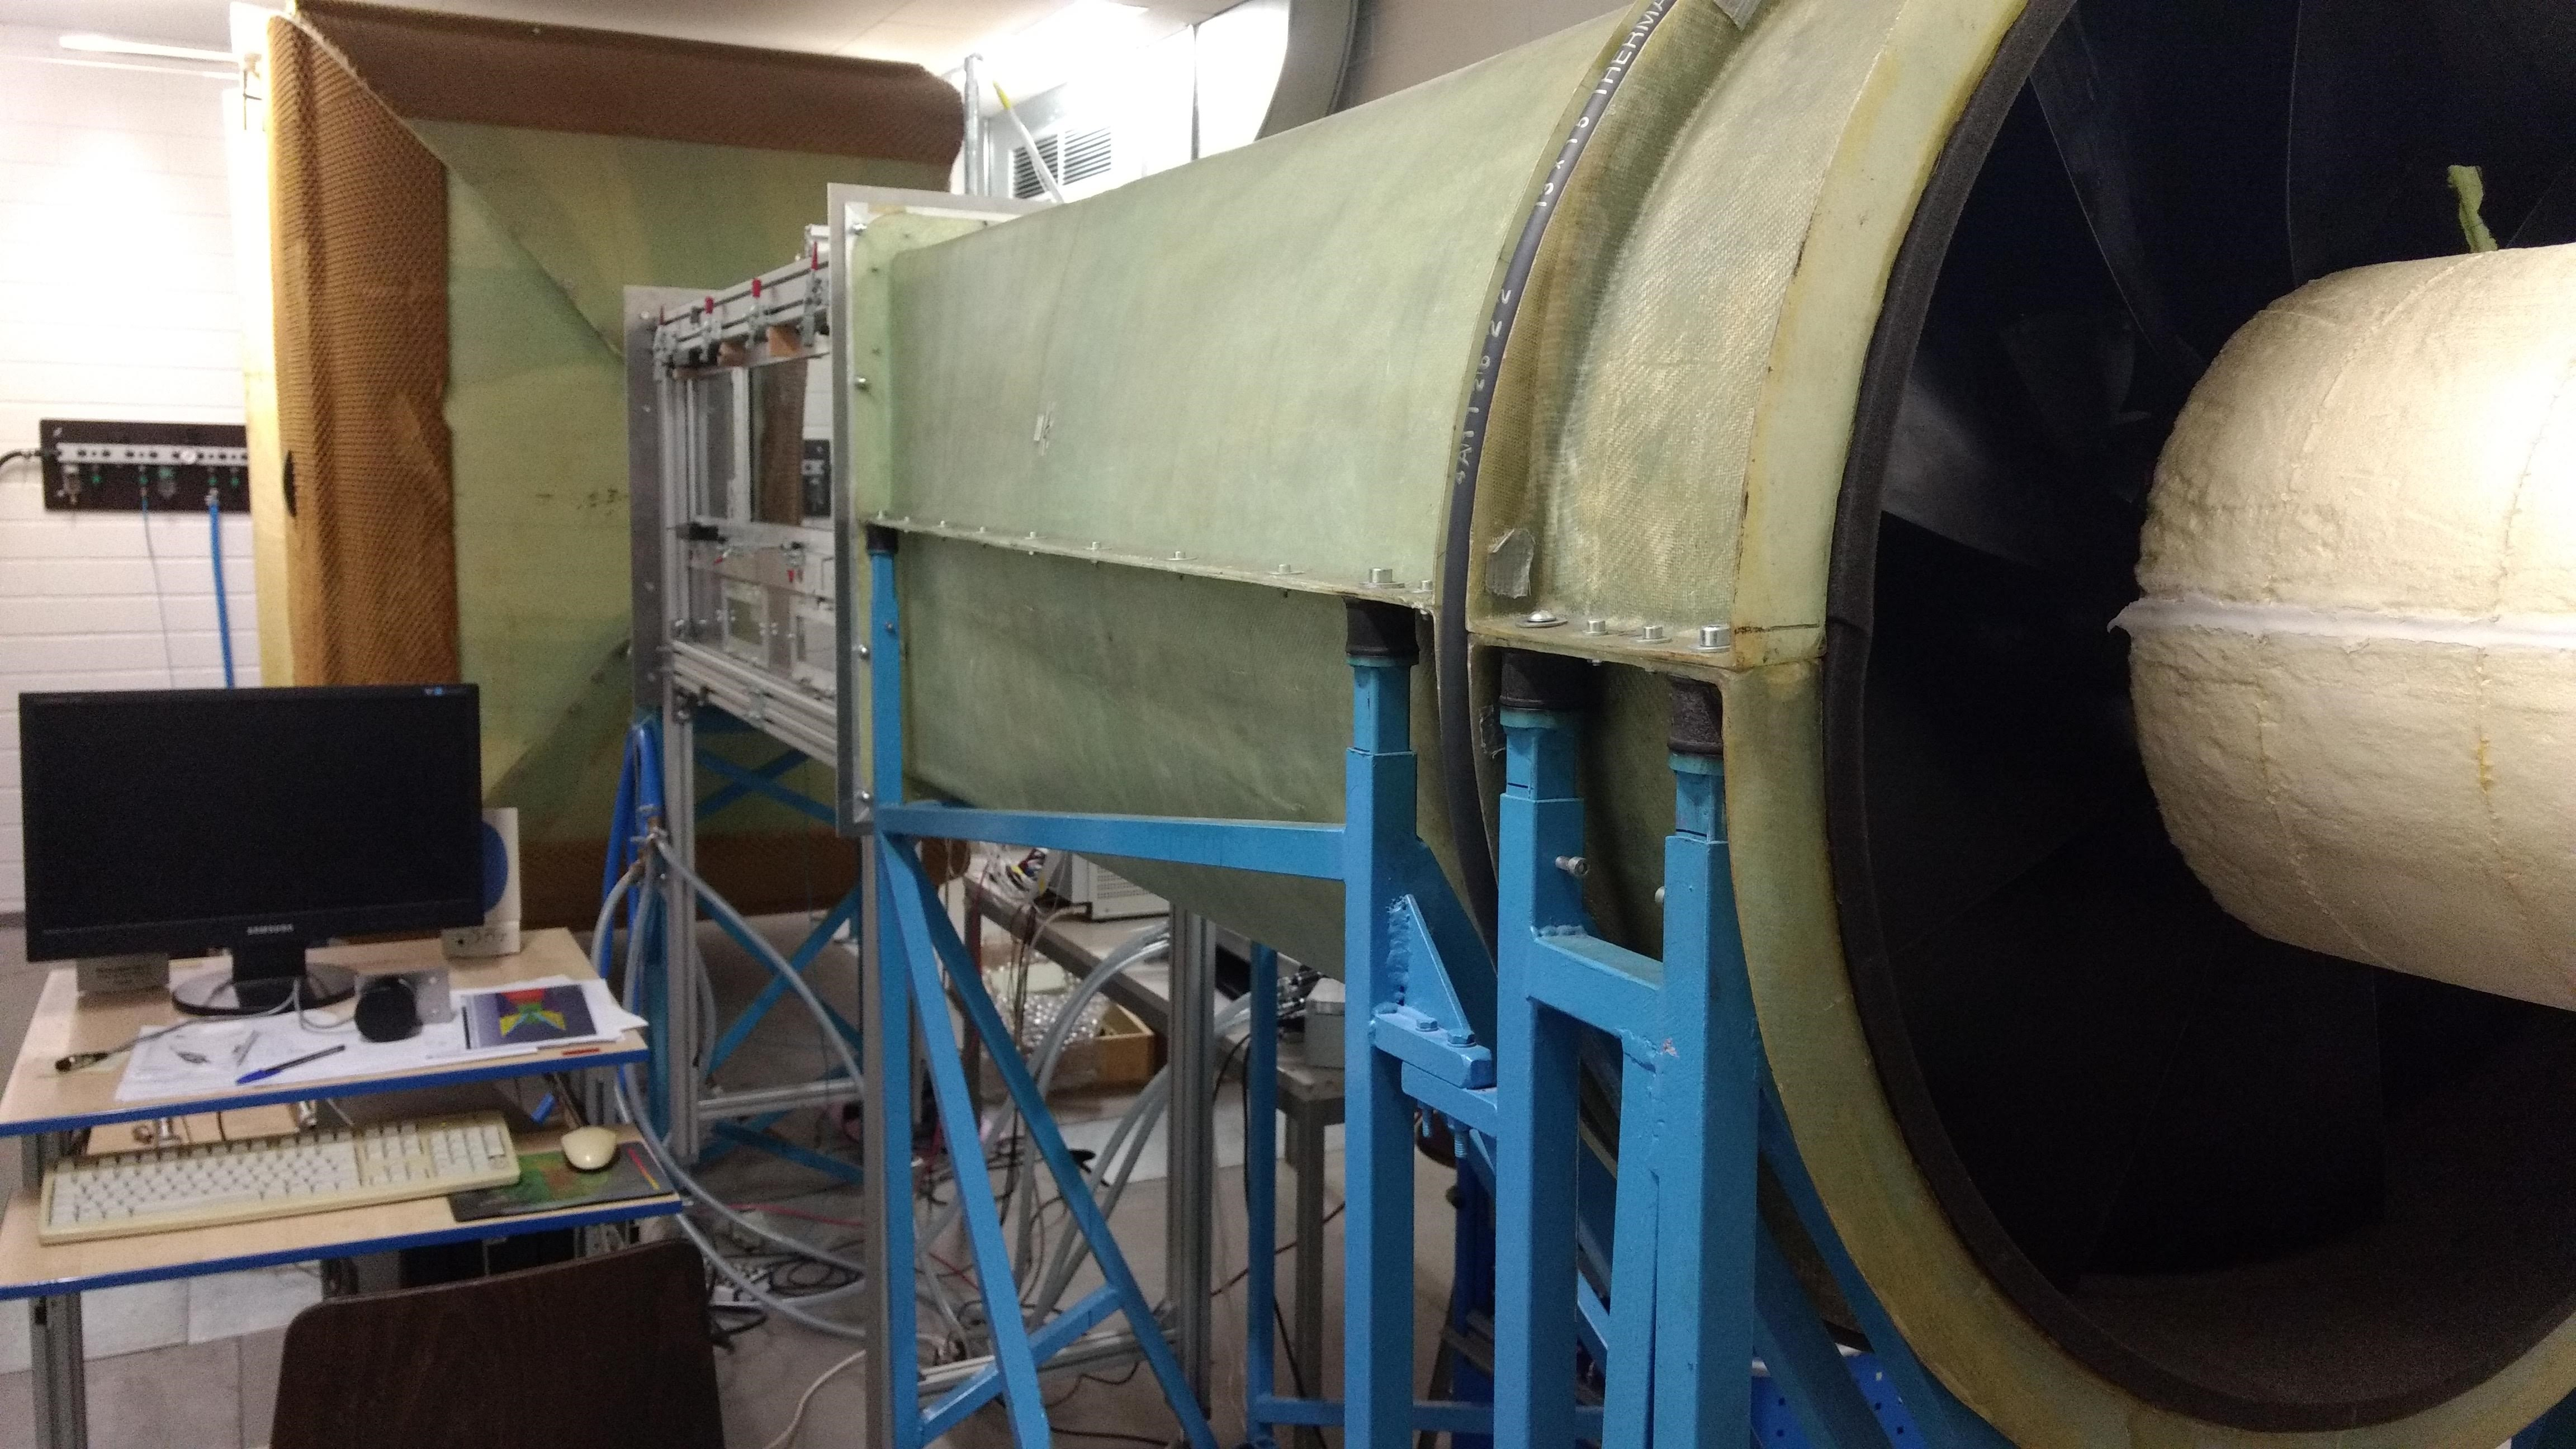
\includegraphics[width=1\textwidth]{windkanal2.jpg}
	\end{subfigure}
	\caption{LNB-ISM TU Braunschweig}
	\label{fig:windkanal}
\end{figure}\\
Testk"orper, die f"ur die Untersuchung eine maximale Anstr"omgeschwindigkeit von \SI{20}{\meter/\second} ben"otigen und die passende Gr"o\ss{}e haben, sind f"ur Versuche in diesem Windkanal geeignet.

\section{Messtechnik (KK)}
Nicht nur bei der Versuchsvorbereitung, sondern auch w"ahrend des Versuchs werden Messger"ate und Einrichtungen ben"otigt, ohne die eine sinnvolle Untersuchung und rechnerische Ermittlungen der Versuchsparameter nicht m"oglich ist.

Hier wird auf die f"ur den Versuch eingesetzten Messmittel und deren Funktionsweisen eingegangen.

\subsection{Messuhr}
Die Messuhr wird f"ur die Messung der L"angendifferenzen oder auch L"angen eingesetzt. Mit einer "ublichen Genauigkeit von \SI{10}{\micro\meter} und einem Messbereich von 5 bis \SI{60}{\milli\meter} eignen sich die Messuhren f"ur Parallelit"ats- und Ebenheitsmessungen.

\subsection{Fischmaul-Sonde}
Die Fischmaul-Sonde ist im Prinzip ein an der Spitze plattgedr"ucktes Pitot-Rohr. Sie eignet sich am besten f"ur Staudruckmessungen an bzw. in angestr"omten Spalten.

\subsection{Statische Sonde}
Die statische Sonde besitzt nur Bohrungen, die tangential zur Str"omung sind und deshalb nur für die Messung des statischen Drucks geeignet sind.
Damit die Bohrungen m"oglichst keinen dynamischen Anteil messen, m"ussen sie sich weit genug entfernt von der Sondenspitze befinden, da in und nach diesem Bereich, die Str"omung umgelenkt wird und lokal nicht mehr tangential zu den Bohrungseintrittsfl"achen steht.

\subsection{Prandtl-Sonde}
Diese Sonde kombiniert die statische Sonde und das Pitot-Rohr.
Die von der seitlichen Bohrungen gemessenen Dr"ucke laufen im inneren System gegen den an der Spitze gemessenen Staudruck.
Somit wird der statische Druck vom Gesamtdruck abgezogen und der dynamische Druck erhalten. Durch weitere Rechnungen ist es m"oglich, mittels dynamischen Drucks die Anstr"omgeschwindigkeiten zu berechnen.

\subsection{Drehzahlmesser}

\subsection{PSI-Anlage}

%%%%%%%%%%%%%%%%%%%%%%%%Modellbeschreibung Tim%%%%%%%%%%%%%%%%%%%%%%%%%%%%%

\section{Modell (TG)}
Die Versuche werden am gleichen Modell duchgef"uhrt, welches im Zuge der Masterarbeit von Bilges \cite{Bilges.2018} entstanden ist. Dieses ist in \abb{fig:DModell} zu sehen.

\begin{figure}[h]
	\centering
	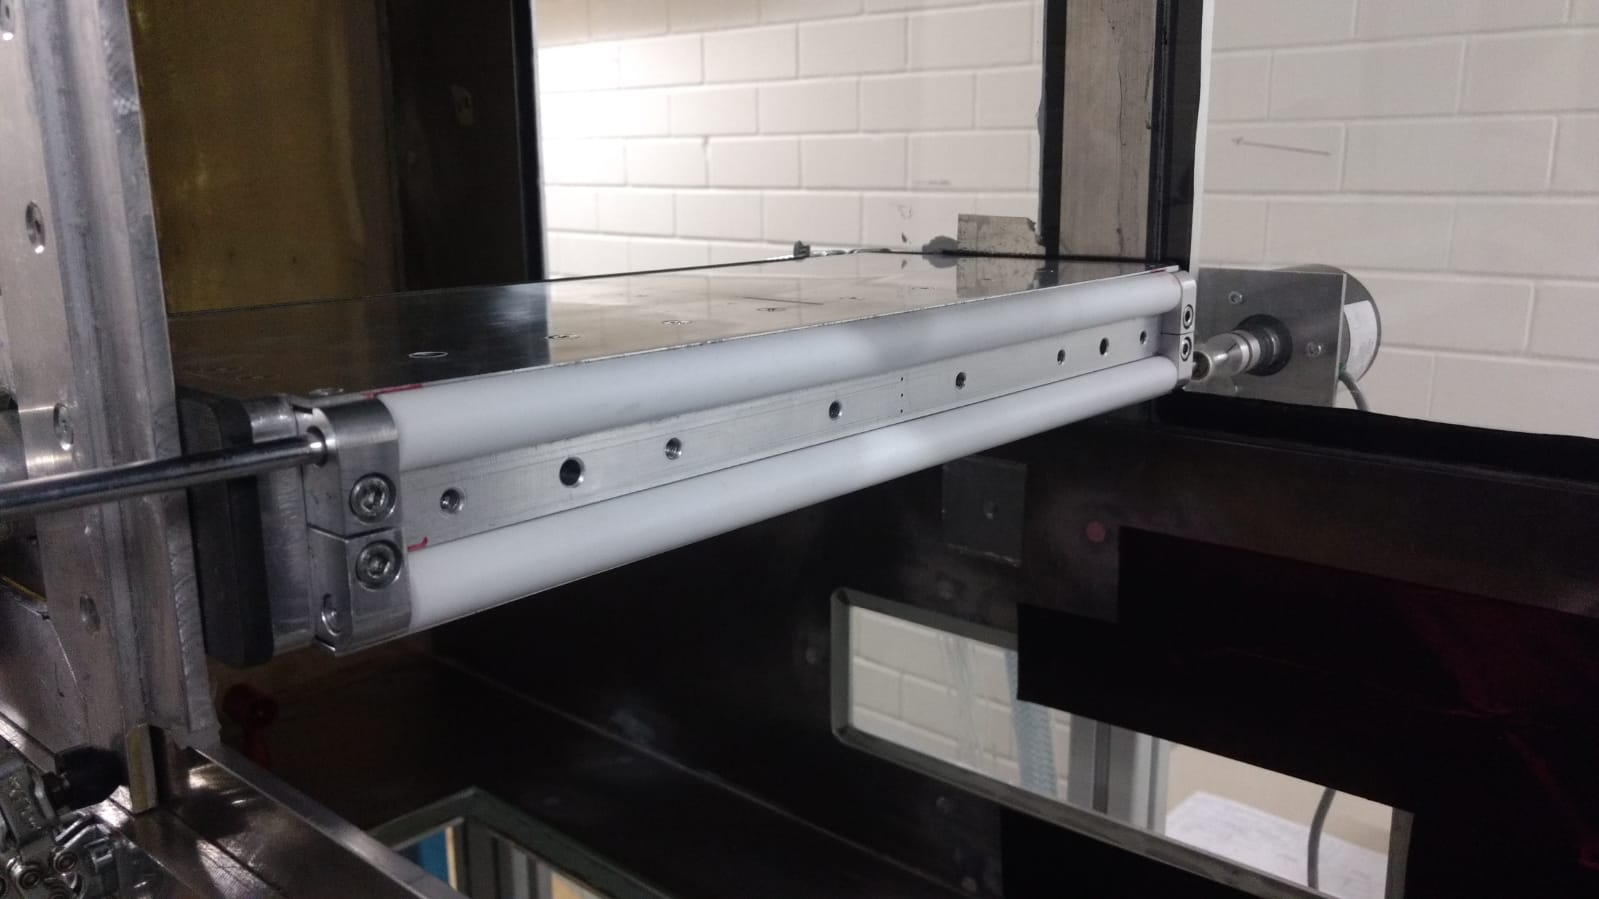
\includegraphics[width=0.8\textwidth]{DModell.jpg}
	\caption{Verwendetes Versuchsmodell mit eingebauten Teflonwalzen. Die Wellen werden seitlich aus dem Windkanal herausgef"uhrt und "uber eine Sicherheitskupplung durch jeweils einen Elektromotor angetrieben.}
	\label{fig:DModell}
\end{figure}

 Dabei handelt es sich um einen D-f"ormigen  Stumpfk"oper folgender Abmessungen. 
\begin{figure}[h]
	\centering
	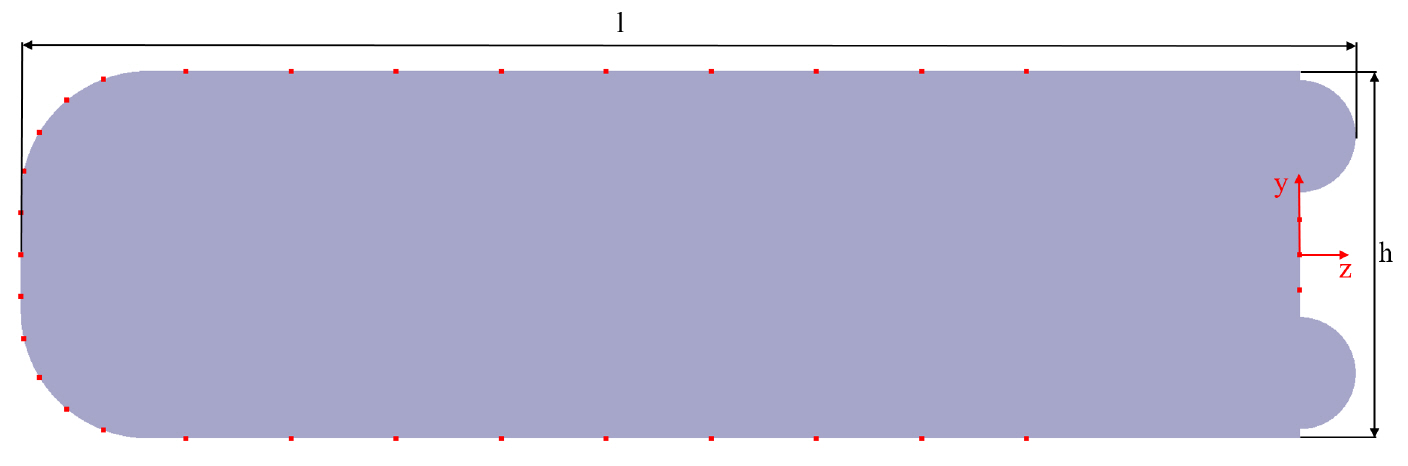
\includegraphics[width=1\textwidth]{ModellGeometrie.jpg}
	\caption{Geometrie des D-Stumpfk"orpers mit eingezeichneten Druckbohrungen \citep{Bilges.2018}}
	\label{fig:ModellGeometrie}
\end{figure}


\begin{figure}[h]
	\centering
	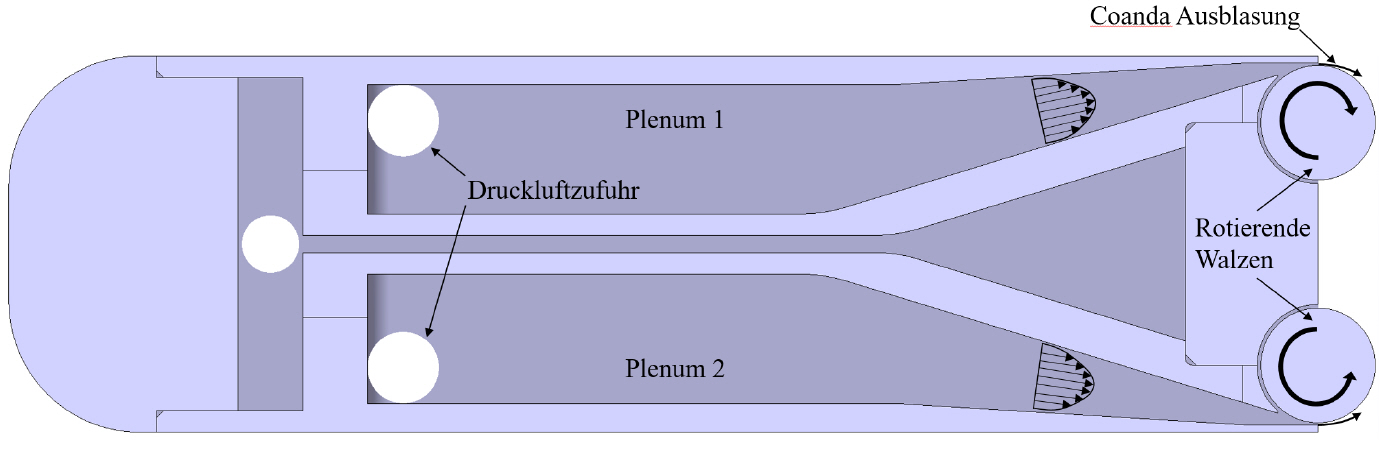
\includegraphics[width=1\textwidth]{SkizzeModell.jpg}
	\caption{Skizze des Versuchsmodells \citep{Bilges.2018}}
	\label{fig:SkizzeModell}
\end{figure}


%%%%%%%%%%%%%%%%%%%%%%Kebria%%%%%%%%%%%%%%%%%%%%%%%%%%%%%%%%%%%%%


\section{Versuchsvorbereitung (KK)}

